\documentclass[a4paper,10pt]{article}
\usepackage[utf8]{inputenc}
\usepackage{amsmath}
\usepackage{xfrac}
%\usepackage[demo]{graphicx}
\usepackage[caption = false]{subfig}
\usepackage{float}
\usepackage[a4paper, total={7.5in, 10in}]{geometry}
\usepackage{longtable}
\usepackage{dcolumn,booktabs}
\usepackage[table]{xcolor}
\usepackage{listings}
\lstset{
breaklines=true
}
%http://tex.stackexchange.com/questions/116534/lstlisting-line-wrapping
\usepackage{hyperref}
\hypersetup{
    colorlinks=true,
    linkcolor=blue,
    citecolor=blue
}

\lstset{language=[77]Fortran,
  basicstyle=\ttfamily,
  keywordstyle=\color{red},
  commentstyle=\color{green},
  morecomment=[l]{!\ }% Comment only with space after !
}

\usepackage{color}
 
\definecolor{codegreen}{rgb}{0,0.6,0}
\definecolor{codegray}{rgb}{0.5,0.5,0.5}
\definecolor{codepurple}{rgb}{0.58,0,0.82}
\definecolor{backcolour}{rgb}{0.95,0.95,0.92}
 
\lstdefinestyle{mystyle}{
    backgroundcolor=\color{backcolour},   
    commentstyle=\color{codegreen},
    keywordstyle=\color{magenta},
    numberstyle=\tiny\color{codegray},
    stringstyle=\color{codepurple},
    basicstyle=\footnotesize,
    breakatwhitespace=false,         
    breaklines=true,                 
    captionpos=b,                    
    keepspaces=true,                 
    numbers=left,                    
    numbersep=5pt,                  
    showspaces=false,                
    showstringspaces=false,
    showtabs=false,                  
    tabsize=2
}
 
\lstset{style=mystyle}

%opening

\title{Homework 5 \\
\textbf{Three Body Problem}}
\author{Arvind Balasubramanian}
\date{}

\begin{document}
\maketitle
\section*{Python code and analysis}
\begin{lstlisting}[language=python]
import numpy as np
import matplotlib.pyplot as plt

### Constants ###########

t_final = 10
dt = 10**(-2.0)

M_sun = 1.0
M_jupiter = 1.0 # 10**(-4)
M_earth = 10**(-6)
# Initial position
x0_sun = 0
y0_sun = 0
x0_jupiter = 5.2
y0_jupiter = 0
x0_earth = 1.0
y0_earth = 0
# Initial velocities
vx0_sun = 0
vy0_sun = 0
vx0_jupiter = 0
vy0_jupiter = 2*np.pi*13.07/30.0
vx0_earth = 0
vy0_earth = 2*np.pi

G = 4*(np.pi**2.0)/M_sun

##### Initializing arrays

time = np.arange(0, t_final + dt, dt)

def acceleration_1(Ms, Mj, pos1s, pos1j, r1s, r1j):
    """
    Function to give acceleration of a mass due to Ms and Mj when its coordinate is pos1s from that of Ms and pos1j from that of Mj and the corresponding distances between them are r1s and r1j
    """
    return - (G*Ms*pos1s/(r1s**3.0)) - (G*Mj*pos1j/(r1j**3.0))

def three_body_problem(time_array):
    """
    Calculates position at a later time using Euler Cromer method
    """

    x_sun = np.zeros(len(time_array))
    x_sun[0] = x0_sun
    y_sun = np.zeros(len(time_array))
    y_sun[0] = y0_sun
    x_jupiter = np.zeros(len(time_array))
    x_jupiter[0] = x0_jupiter
    y_jupiter = np.zeros(len(time_array))
    y_jupiter[0] = y0_jupiter

    x_earth = np.zeros(len(time_array))
    x_earth[0] = x0_earth
    y_earth = np.zeros(len(time_array))
    y_earth[0] = y0_earth

    vx_sun = np.zeros(len(time_array))
    vx_sun[0] = vx0_sun
    vy_sun = np.zeros(len(time_array))
    vy_sun[0] = vy0_sun

    vx_jupiter = np.zeros(len(time_array))
    vx_jupiter[0] = vx0_jupiter
    vy_jupiter = np.zeros(len(time_array))
    vy_jupiter[0] = vy0_jupiter

    vx_earth = np.zeros(len(time_array))
    vx_earth[0] = vx0_earth
    vy_earth = np.zeros(len(time_array))
    vy_earth[0] = vy0_earth

    for i in range(len(time_array)-1):
        r_sj = np.sqrt(((x_sun[i] - x_jupiter[i])**2.0) + ((y_sun[i] - y_jupiter[i])**2.0))
        r_se = np.sqrt(((x_sun[i] - x_earth[i])**2.0) + ((y_sun[i] - y_earth[i])**2.0))
        r_je = np.sqrt(((x_earth[i] - x_jupiter[i])**2.0) + ((y_earth[i] - y_jupiter[i])**2.0))

        vx_sun[i+1] = vx_sun[i] + dt*acceleration_1(M_earth, M_jupiter, (x_sun[i] -a x_earth[i]), (x_sun[i] - x_jupiter[i]), r_se, r_sj)
        vy_sun[i+1] = vy_sun[i] + dt*acceleration_1(M_earth, M_jupiter, (y_sun[i] - y_earth[i]), (y_sun[i] - y_jupiter[i]), r_se, r_sj)
        vx_jupiter[i+1] = vx_jupiter[i] + dt*acceleration_1(M_sun, M_earth, (x_jupiter[i] - x_sun[i]), (x_jupiter[i] - x_earth[i]), r_sj, r_je)
        vy_jupiter[i+1] = vy_jupiter[i] + dt*acceleration_1(M_sun, M_earth, (y_jupiter[i] - y_sun[i]), (y_jupiter[i] - y_earth[i]), r_sj, r_je)
        vx_earth[i+1] = vx_earth[i] + dt*acceleration_1(M_sun, M_jupiter, (x_earth[i] - x_sun[i]), (x_earth[i] - x_jupiter[i]), r_se, r_je)
        vy_earth[i+1] = vy_earth[i] + dt*acceleration_1(M_sun, M_jupiter, (y_earth[i] - y_sun[i]), (y_earth[i] - y_jupiter[i]), r_se, r_je)

        x_sun[i+1] = x_sun[i] + dt*vx_sun[i+1]
        y_sun[i+1] = y_sun[i] + dt*vy_sun[i+1]
        x_jupiter[i+1] = x_jupiter[i] + dt*vx_jupiter[i+1]
        y_jupiter[i+1] = y_jupiter[i] + dt*vy_jupiter[i+1]
        x_earth[i+1] = x_earth[i] + dt*vx_earth[i+1]
        y_earth[i+1] = y_earth[i] + dt*vy_earth[i+1]

    return x_sun, y_sun, x_jupiter, y_jupiter, x_earth, y_earth

x_sun, y_sun, x_jupiter, y_jupiter, x_earth, y_earth = three_body_problem(time)

\end{lstlisting}

\pdfsuppresswarningpagegroup=1

\vspace{80pt}

\section*{Plotting trajectories for the three bodies}
The plots have been made for the following values of $\alpha = \frac{\text{M}_{sun}}{\text{M}_{jupiter}}$ :

\begin{longtable}{c c c c}

(a) : 10$^{-4}$ & (b) : 10$^{-1}$ & (c) : 0.5 & (d) : 1.0
 
\end{longtable}

And the value of $\frac{\text{M}_{sun}}{\text{M}_{earth}}$ is 10$^{-6}$ for all of these cases.

\begin{figure}
\subfloat[]{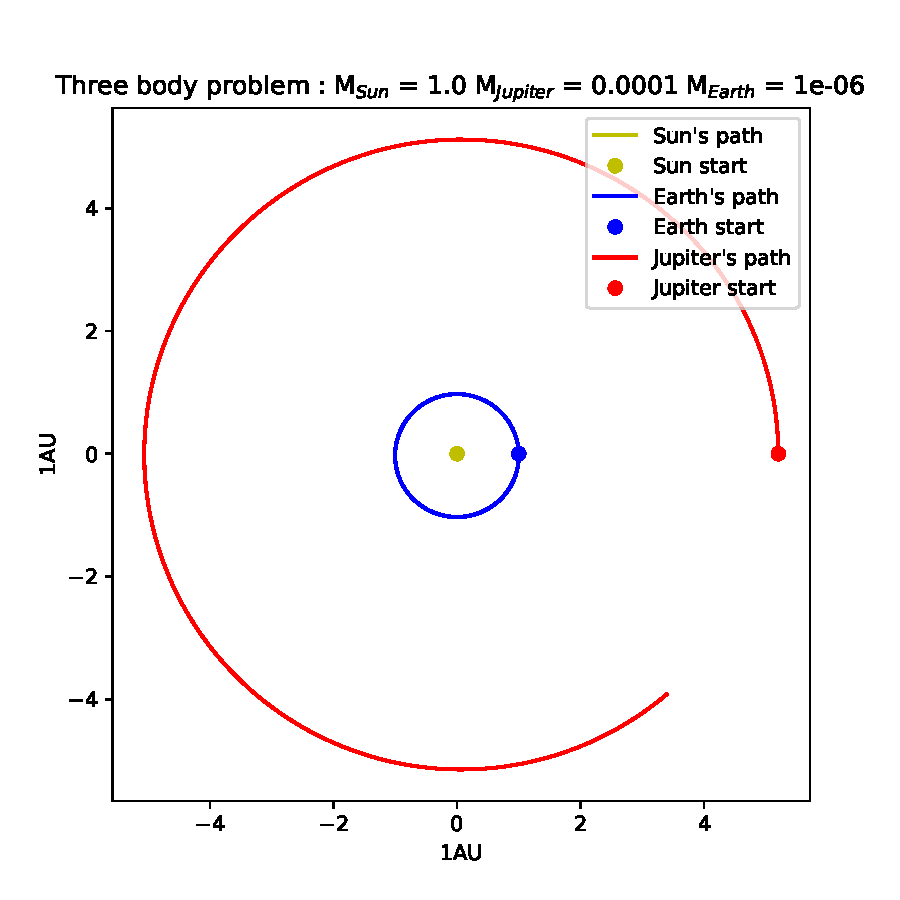
\includegraphics[width = 0.5\textwidth]{Alpha_minus_four}} 
\subfloat[]{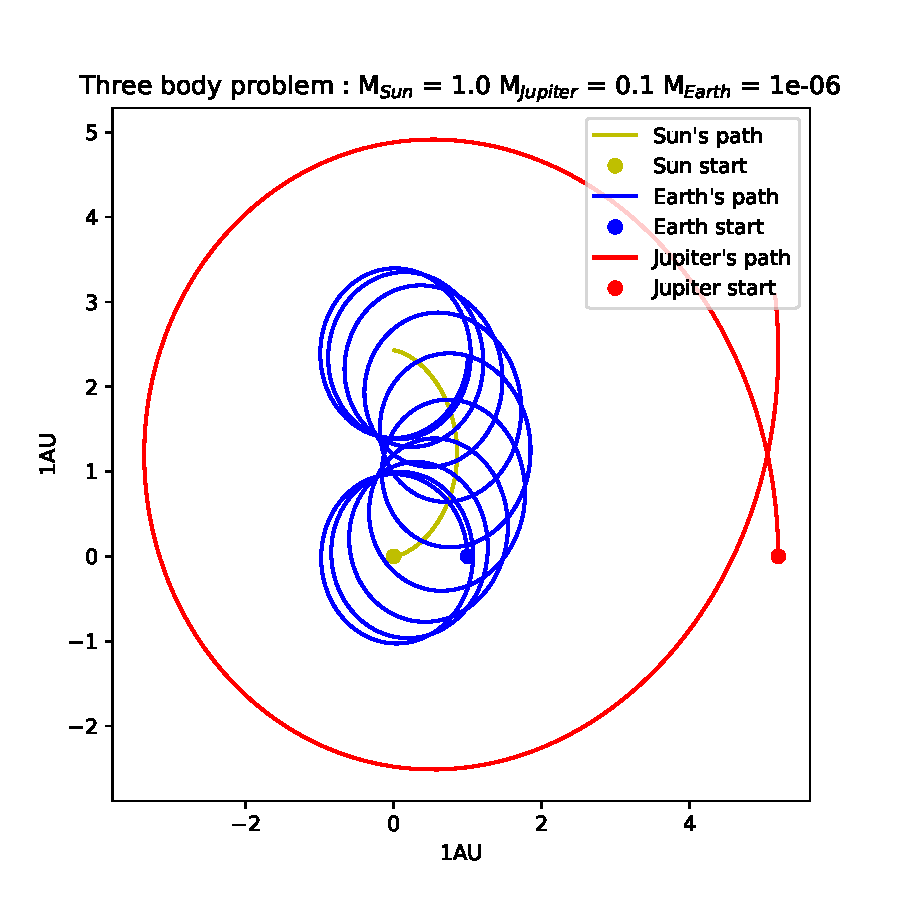
\includegraphics[width = 0.5\textwidth]{Alpha_minus_one}}\\ 
\subfloat[]{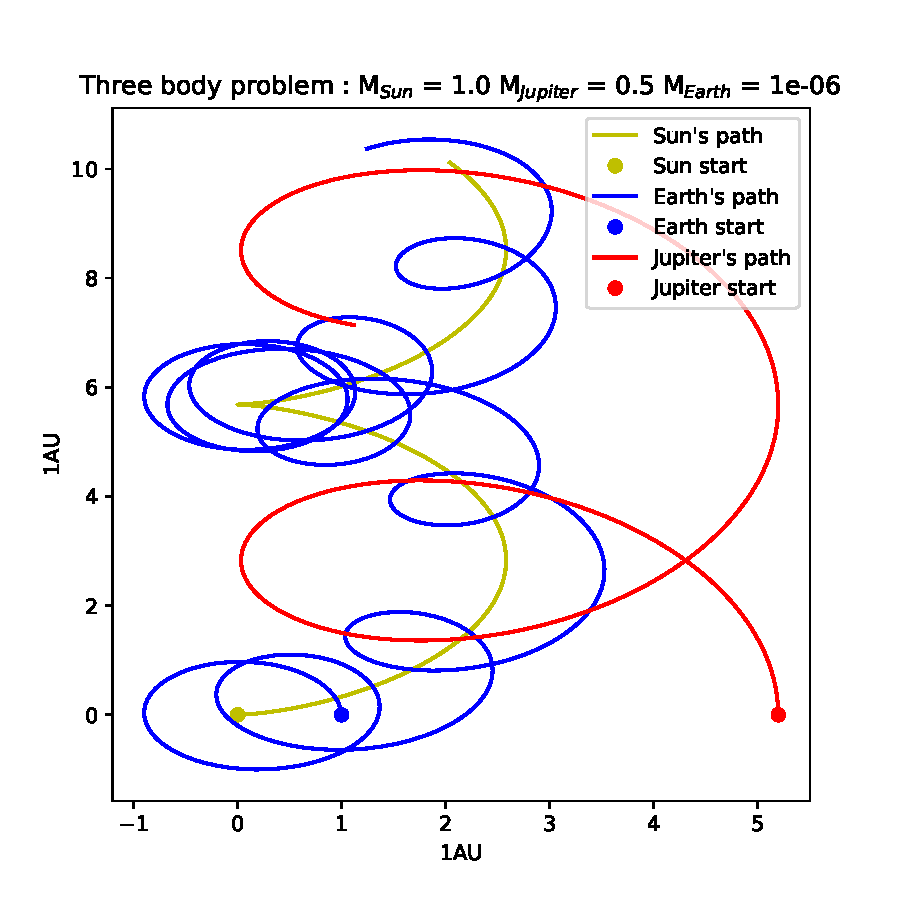
\includegraphics[width = 0.5\textwidth]{Alpha_half}} 
\subfloat[]{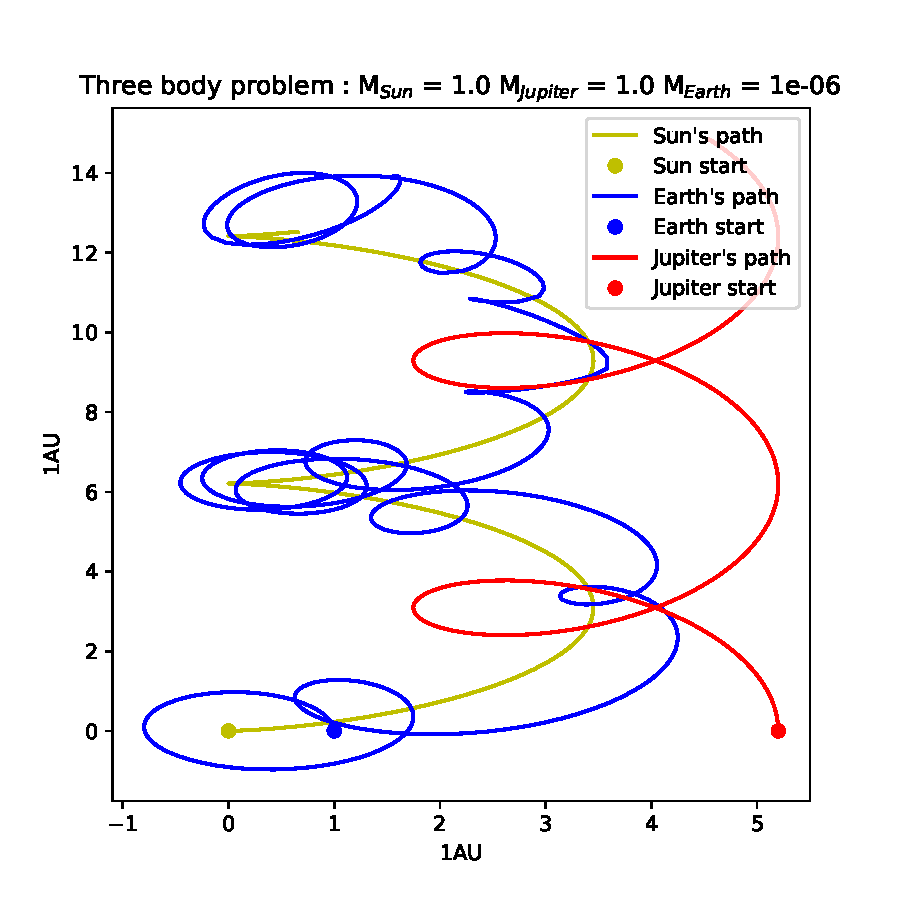
\includegraphics[width = 0.5\textwidth]{Alpha_one}} 
\end{figure}


\end{document}
